%https://gateoverflow.in/118343/gate-cse-2017-set-2-question-6?show=118224
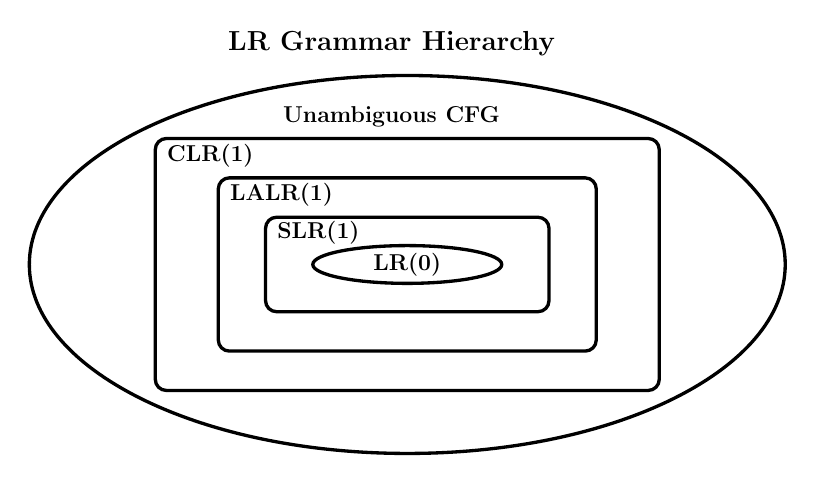
\begin{tikzpicture}[scale = 0.4,transform shape]

\draw[very thick] (0,0) ellipse (12cm and 6cm);

\draw[rounded corners,very thick] (-8,-4) rectangle (8,4);

\draw[rounded corners,very thick] (-6,-2.75) rectangle (6,2.75);

\draw[rounded corners,very thick] (-4.5,-1.5) rectangle (4.5,1.5);
\draw[very thick] (0,0) ellipse (3cm and 0.60cm);

\node[] at (0,0) {\huge{$\textbf{LR(0)}$}};
\node[right] at (-4.25,1) {\huge{$\textbf{SLR(1)}$}};
\node[right] at (-5.75,2.20) {\huge{$\textbf{LALR(1)}$}};
\node[right] at (-7.75,3.45) {\huge{$\textbf{CLR(1)}$}};
\node[above] at (-0.5,4.25) {\huge{$\textbf{Unambiguous CFG}$}};
\node[above] at (-0.5,6.5) {\Huge{$\textbf{LR Grammar Hierarchy}$}};
\end{tikzpicture}